\documentclass[12pt,a4paper]{article}
\usepackage[margin=1in]{geometry}
\usepackage[latin1]{inputenc}
\usepackage{graphicx}
\usepackage{amsmath}
\usepackage{amsfonts}
\usepackage{amssymb}
\usepackage{url}
\usepackage{booktabs}
\usepackage{tikz}
\usepackage[compact,explicit]{titlesec}

\usetikzlibrary{positioning, shapes, decorations.text}

\begin{document}

\begin{figure}[ht]
\centering
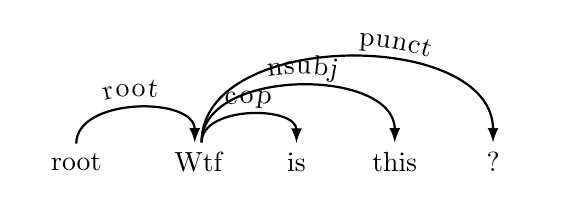
\begin{tikzpicture}[
mynode/.style={rectangle,
  fill=white!70,
  text width=1cm,
  align=center,
},
mypostaction/.style 2 args={
  decoration={
    text align={
      left indent=#1},
      text along path, 
      text={#2}
    },
  decorate
},
>=latex
]

\node[mynode] (r)
    {root};
\node[mynode, right= 0.3cm of r] (wtf)
    {Wtf};
\node[mynode, right= 0cm of wtf] (is)
    {is};
\node[mynode, right= 0cm of is] (this)
    {this};
\node[mynode, right= 0cm of this] (qm)
    {?};

\draw[->,thick,black] (r.north) to[out=90,in=90,looseness=1] (wtf.100);
\path[postaction={mypostaction={0.6cm}{root}, /pgf/decoration/raise=1.5mm}] (r.north) to[out=90,in=90,looseness=1] (wtf.100);

\draw[->,thick,black] (wtf.80) to[out=90,in=90,looseness=1] (is.north);
\path[postaction={mypostaction={0.5cm}{cop}, /pgf/decoration/raise=1.5mm}] (wtf.80) to[out=90,in=90,looseness=1] (is.north);

\draw[->,thick,black] (wtf.80) to[out=90,in=90,looseness=1] (this.north);
\path[postaction={mypostaction={1.2cm}{nsubj}, /pgf/decoration/raise=1.5mm}] (wtf.80) to[out=90,in=90,looseness=1] (this.north);

\draw[->,thick,black] (wtf.80) to[out=90,in=90,looseness=1] (qm.north);
\path[postaction={mypostaction={2.5cm}{punct}, /pgf/decoration/raise=1.5mm}] (wtf.80) to[out=90,in=90,looseness=1] (qm.north);
\end{tikzpicture}
\caption{Golden parse}
\label{Fig2}
\end{figure}

\begin{figure}[ht]
\centering
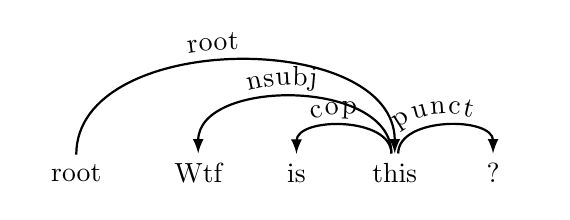
\begin{tikzpicture}[
mynode/.style={rectangle,
  fill=white!70,
  text width=1cm,
  align=center,
},
mypostaction/.style 2 args={
  decoration={
    text align={
      left indent=#1},
      text along path, 
      text={#2}
    },
  decorate
},
>=latex
]

\node[mynode] (r)
    {root};
\node[mynode, right= 0.3cm of r] (wtf)
    {Wtf};
\node[mynode, right= 0cm of wtf] (is)
    {is};
\node[mynode, right= 0cm of is] (this)
    {this};
\node[mynode, right= 0cm of this] (qm)
    {?};

\draw[->,thick,black] (r.north) to[out=90,in=90,looseness=1] (this.90);
\path[postaction={mypostaction={2cm}{root}, /pgf/decoration/raise=1.5mm}] (r.north) to[out=90,in=90,looseness=1] (this.100);

\draw[->,thick,black] (this.100) to[out=90,in=90,looseness=1] (is.north);
\path[postaction={mypostaction={0.4cm}{cop}, /pgf/decoration/raise=1.5mm}] (is.north) to[out=90,in=90,looseness=1] (this.100);

\draw[->,thick,black] (this.100) to[out=90,in=90,looseness=1] (wtf.north);
\path[postaction={mypostaction={1cm}{nsubj}, /pgf/decoration/raise=1.5mm}] (wtf.north) to[out=90,in=90,looseness=1] (this.100);

\draw[->,thick,black] (this.80) to[out=90,in=90,looseness=1] (qm.north);
\path[postaction={mypostaction={0.2cm}{punct}, /pgf/decoration/raise=1.5mm}] (this.80) to[out=90,in=90,looseness=1] (qm.north);
\end{tikzpicture}
\caption{Our parse}
\label{Fig2}
\end{figure}

\end{document}
